%====================================================================================
\section{Segundo Teorema del Bienestar}
%====================================================================================

\begin{frame}{Segundo Teorema del Bienestar}
	\begin{itemize}
		\item Si tomamos una asignación eficiente, ¿podemos garantizar que esta sea de equilibrio competitivo?
		\item ``Cuando las preferencias de ambos consumidores son convexas, contínuas y monótonas, cualquier asignación óptimo de Pareto puede ser de equilibrio walrasiano, si se permite las adecuadas transferencias entre los consumidores''.
	\end{itemize}
\end{frame}
%------------------------------------------------
\begin{frame}{Segundo Teorema del Bienestar}
$X$	es una asignación óptima obtenida por equilibrio competitivo desde la dotación $W$.
	\begin{center}
		\begin{tikzpicture}[transform canvas={scale=0.63}]
	% Formato de CAJA
		\draw[->] (0.5,0.5) node[align=center, below left] {\footnotesize $O_B$} -- (0.5,4.5) node[align=center, above] {\footnotesize $x_{2}^{B}$};
		\draw[->] (0.5,0.5) -- (8.5,0.5) node[align=center, right] {\footnotesize $x_{1}^{B}$};
	
		% Curvas de indiferencia1
			% Agente B
				\draw  [red] (0.6,4) ..controls (1.4,1.4) and (1.74,1) .. (6,0.6);
				\draw  [red] (1,4.3) ..controls (1.7,2.1) and (2,1.6) .. (6.3,1);
				\draw  [red] (1.6,4.6) ..controls (2.1,3.2) and (1.74,2.2) .. (6.7,1.4);
			
			% Flechas
				\node[draw, single arrow,
						minimum height=30mm, minimum width=1mm,
						single arrow head extend=1.5mm,
						anchor=west, red, fill=red, scale=0.5, rotate=50] at (2.7,2.7) {};
	% Flecha
		\node[draw, single arrow,
				minimum height=33mm, minimum width=8mm,
				single arrow head extend=2mm,
				anchor=west,] at (8,2) {Rotando 180$^{\circ}$};
	
	% Formato de CAJA rotado
		\draw[->] (18,4) node[align=center, above right] {\footnotesize $O_B$} -- (10,4) node[align=center, left] {\footnotesize $x_{1}^{B}$};
		\draw[->] (18,4) -- (18,0) node[align=center, below] {\footnotesize $x_{2}^{B}$};
	
		% Curvas de indiferencia1
			% Agente B
				\draw [red] (12,3.9) .. controls (16.76,3.5) and (17.1,3.1) .. (17.9,0.5);
				\draw [red] (11.7,3.5) .. controls (16.5,2.9) and (16.8,2.4) .. (17.3,0.2);
				\draw [red] (11.3,3.1) .. controls (16.76,2.3) and (16.4,1.3) .. (16.6,-0.1);
			
			% Flechas
				\node[draw, single arrow,
						minimum height=30mm, minimum width=1mm,
						single arrow head extend=1.5mm,
						anchor=west, red, fill=red, scale=0.5, rotate=-130] at (15.7,1.8) {};
\end{tikzpicture}
	\end{center}
\end{frame}
%------------------------------------------------
\begin{frame}{Segundo Teorema del Bienestar}
¿Puede obtenerse esta asignación $N$ desde $W$? 
	\begin{center}
		\begin{tikzpicture}[scale=1]
	% Formación de la caja
	% Consumidor A
	\draw[->] (0.5,0.5) node[align=center, below left] {\footnotesize $O_A$} -- (0.5,4.5) node[align=center, above] {\footnotesize $x_{2}^{A}$};
	\draw[->] (0.5,0.5) -- (8.5,0.5) node[align=center, right] {\footnotesize $x_{1}^{A}$};
	
	\draw (6,0.5) node[below] {\footnotesize $x_{1}^{A}$};
	\draw (0.5,2) node[left] {\footnotesize $x_{2}^{A}$};
	
	% Llaves
	\draw [decorate,decoration={brace,amplitude=5pt},xshift=-4pt,yshift=0pt] (6.1,-0.05) -- (0.7,-0.05);
	\node [right] at (3,-0.4) {$w_{1}^{A}$};
	
	\draw [decorate,decoration={brace,amplitude=5pt},xshift=-4pt,yshift=0pt] (-0.05,0.5) --(-0.05,2);
	\node [left] at (-0.3,1.27) {$w_{2}^{A}$};
\end{tikzpicture}
	\end{center}
\end{frame}
%------------------------------------------------
\begin{frame}{Segundo Teorema del Bienestar}
¿Puede obtenerse esta asignación $N$ desde $W$? $\longrightarrow$ No, porque ya hay un sistema de precios y una dotación inicial
	\begin{center}
		\begin{tikzpicture}[transform canvas={scale=0.6}]
	% Consumidor B sin rotar
		\draw[->] (0.5,0.5) node[align=center, below left] {\footnotesize $O_B$} -- (0.5,4.5) node[align=center, above] {\footnotesize $x_{2}^{B}$};
		\draw[->] (0.5,0.5) -- (8.5,0.5) node[align=center, right] {\footnotesize $x_{1}^{B}$};
	
		\draw (2,0.5) node[below] {\footnotesize $x_{1}^{B}$};
		\draw (0.5,2.5) node[left] {\footnotesize $x_{2}^{B}$};
	
		% Llaves
			\draw [decorate,decoration={brace,amplitude=5pt},xshift=-4pt,yshift=0pt] (2,-0.05) -- (0.7,-0.05);
			\node [right] at (0.9,-0.4) {$w_{1}^{B}$};
			
			\draw [decorate,decoration={brace,amplitude=5pt},xshift=-4pt,yshift=0pt] (-0.05,0.5) --(-0.05,2.5);
			\node [left] at (-0.3,1.55) {$w_{2}^{B}$};
	
	% Flecha
		\node[draw, single arrow,
		minimum height=33mm, minimum width=8mm,
		single arrow head extend=2mm,
		anchor=west,] at (8,2) {Rotando 180$^{\circ}$};
	
	% Consumidor B con rotación
		\draw[->] (18,4) node[align=center, above right] {\footnotesize $O_B$} -- (10,4) node[align=center, left] {\footnotesize $x_{1}^{B}$};
		\draw[->] (18,4) -- (18,0) node[align=center, below] {\footnotesize $x_{2}^{B}$};
		
		\draw (16,4) node[above] {\footnotesize $x_{1}^{B}$};
		\draw (18,2) node[right] {\footnotesize $x_{2}^{B}$};
		
		% Llaves
			\draw [decorate,decoration={brace,amplitude=5pt},xshift=-4pt,yshift=0pt] (16.2,4.6) --(18.2,4.6);
			\node [right] at (16.78,5.1) {$w_{1}^{B}$};
			
			\draw [decorate,decoration={brace,amplitude=5pt},xshift=-4pt,yshift=0pt] (18.8,4) --(18.8,2);
			\node [right] at (18.8,3.05) {$w_{2}^{B}$};
\end{tikzpicture}
	\end{center}
\end{frame}
%------------------------------------------------
\begin{frame}{Segundo Teorema del Bienestar}
Pero si puede obtenerse desde $\theta$
	\begin{center}
		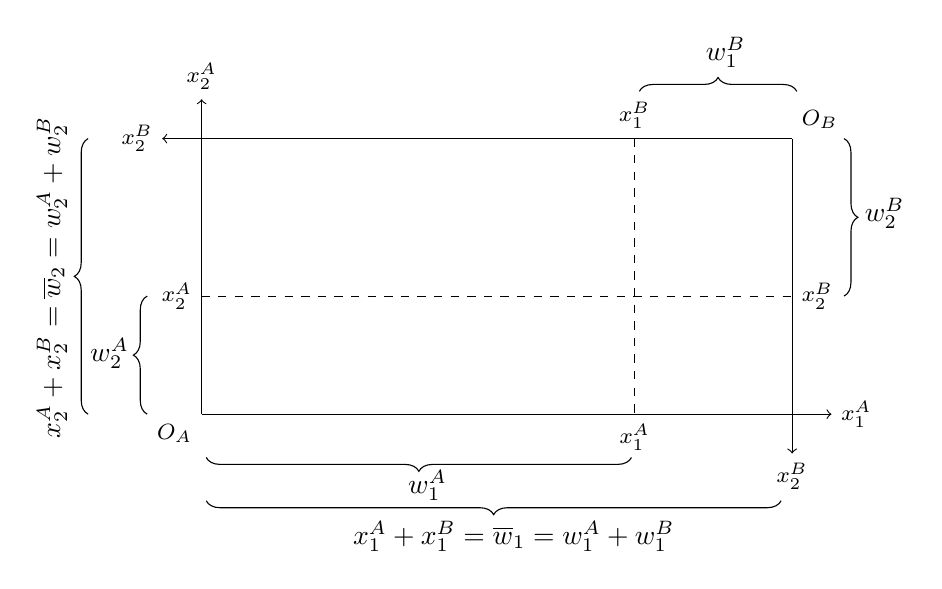
\begin{tikzpicture}[scale=1]
	% Formación de la caja
		% Consumidor A
			\draw[->] (0.5,0.5) node[align=center, below left] {\footnotesize $O_A$} -- (0.5,4.5) node[align=center, above] {\footnotesize $x_{2}^{A}$};
			\draw[->] (0.5,0.5) -- (8.5,0.5) node[align=center, right] {\footnotesize $x_{1}^{A}$};
	
		%Consumidor B
			\draw[->] (8,4) node[align=center, above right] {\footnotesize $O_B$} -- (0,4) node[align=center, left] {\footnotesize $x_{2}^{B}$};
			\draw[->] (8,4) -- (8,0) node[align=center, below] {\footnotesize $x_{2}^{B}$};
	
	% Intersección de una dotación
		\draw[dashed] (6,4) node[above] {\footnotesize $x_{1}^{B}$} -- (6,0.5) node[below] {\footnotesize $x_{1}^{A}$};
		\draw[dashed] (0.5,2) node[left] {\footnotesize $x_{2}^{A}$} -- (8,2)node[right] {\footnotesize $x_{2}^{B}$};
	
	% Llaves
		\draw [decorate,decoration={brace,amplitude=5pt},xshift=-4pt,yshift=0pt] (6.1,-0.05) -- (0.7,-0.05);
		\node [right] at (3,-0.4) {$w_{1}^{A}$};
	
		\draw [decorate,decoration={brace,amplitude=5pt},xshift=-4pt,yshift=0pt] (6.2,4.6) --(8.2,4.6);
		\node [right] at (6.78,5.1) {$w_{1}^{B}$};
		
		\draw [decorate,decoration={brace,amplitude=5pt},xshift=-4pt,yshift=0pt] (-0.05,0.5) --(-0.05,2);
		\node [left] at (-0.3,1.27) {$w_{2}^{A}$};
		
		\draw [decorate,decoration={brace,amplitude=5pt},xshift=-4pt,yshift=0pt] (8.8,4) --(8.8,2);
		\node [right] at (8.8,3.05) {$w_{2}^{B}$};
		
		\draw [decorate,decoration={brace,amplitude=5pt},xshift=-4pt,yshift=0pt] (8,-0.6) -- (0.7,-0.6);
		\node [right] at (2.3,-1.05) {$x_{1}^{A}+x_{1}^{B}=\overline{w}_1=w_{1}^{A}+w_{1}^{B}$};
		
		\draw [decorate,decoration={brace,amplitude=5pt},xshift=-4pt,yshift=0pt] (-0.8,0.5) --(-0.8,4);
		\node [left,rotate=90] at (-1.4,4.4) {$x_{2}^{A}+x_{2}^{B}=\overline{w}_2=w_{2}^{A}+w_{2}^{B}$};
\end{tikzpicture}
	\end{center}
\end{frame}
%------------------------------------------------
\begin{frame}{Segundo Teorema del Bienestar}
A través de un nuevo sistema de precios y una nueva dotación inicial
	\begin{center}
		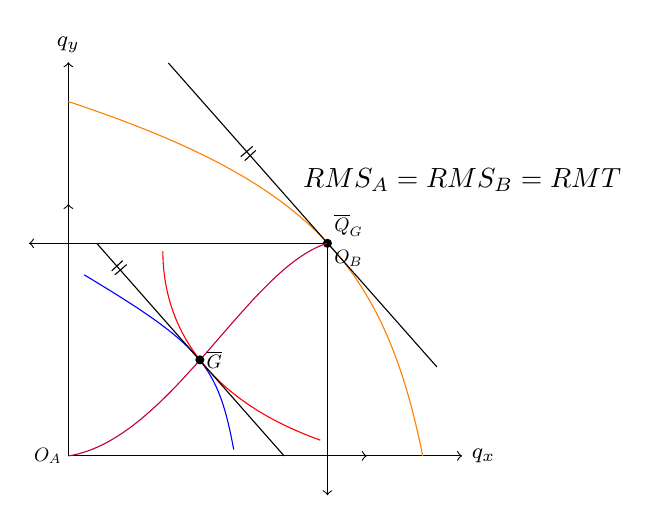
\begin{tikzpicture}
	% FPP
		% Ejes
			\draw[->] (10,0)-- (10,5) node[align=center, above] {\footnotesize $q_{y}$};
			\draw[->] (10,0) -- (15,0) node[align=center, right] {\footnotesize $q_{x}$};
		% Curva
			\draw [orange] (10,4.5) ..controls (13,3.5) and (14,2.5) .. (14.5,0);
			
	% Minicaja
		% Intersección
			\draw [<->] (9.5,2.7) -- (13.29,2.7) node [below right, scale=0.7] {$O_B$} -- (13.29,-0.5);
			\draw [<->] (10,3.2) -- (10,0) node [left, scale=0.7] {$O_A$} -- (13.79,0);
		% Puntos
			\draw[black, fill=black] (13.29,2.7) circle[radius=0.05] node [above right, scale=0.7] {$\overline{Q}_G$};
		% Curva de contrato
			\draw [purple] (10,0) ..controls (11.29,0.2) and (12.29,2.4) .. (13.29,2.7);
			\draw [blue] (10.2,2.3) ..  controls (11.7,1.4) and (11.9,1.15) .. (12.1,0.08);
			\draw [red] (11.2,2.6) ..  controls (11.2,1.6) and (11.8,0.7) .. (13.2,0.2);
		% Pendientes
			\draw (11.27,4.99) -- (14.68,1.13);
			\draw (10.36,2.7) -- (12.74,0);
		% Símbolo de paraleleas
			\draw (10.55,2.35) -- (10.69,2.48);
			\draw (10.59,2.3) -- (10.74,2.43);
			
			\draw (12.19,3.8) -- (12.34,3.93);
			\draw (12.24,3.75) -- (12.38,3.88);
		% 	Etqiueta
			\draw (15, 3.5) node {$RMS_A = RMS_B = RMT$};
		% Punto
			\draw[black, fill=black] (11.67,1.22) circle[radius=0.05] node [right, scale=0.7] {$\overline{G}$};
\end{tikzpicture}
	\end{center}
\end{frame}
%------------------------------------------------
\begin{frame}{Implicancia del Segundo Teorema del Bienestar}
	\begin{itemize}
		\item Se pueden \textbf{\textit{separar los problemas de}} distribución de los problemas de eficiencia.
		
		\item El mercado permite conseguir cualquier asignación de recursos que se desee: es \textbf{\textit{neutral desde el punto de vista distributivo}}.
		
		\item \textbf{\textit{Contenido normativo importante: Todo OP}} se puede sostener por un sistema de precios dada una redistribución adecuada de las dotaciones iniciales (implicancias para la Política Económica).
	\end{itemize}
\end{frame}